\pagebreak
\pagestyle{semifancy}
\chapter*{Függelék}
\addcontentsline{toc}{chapter}{Függelék}

\begin{figure}[H]
    \centering
    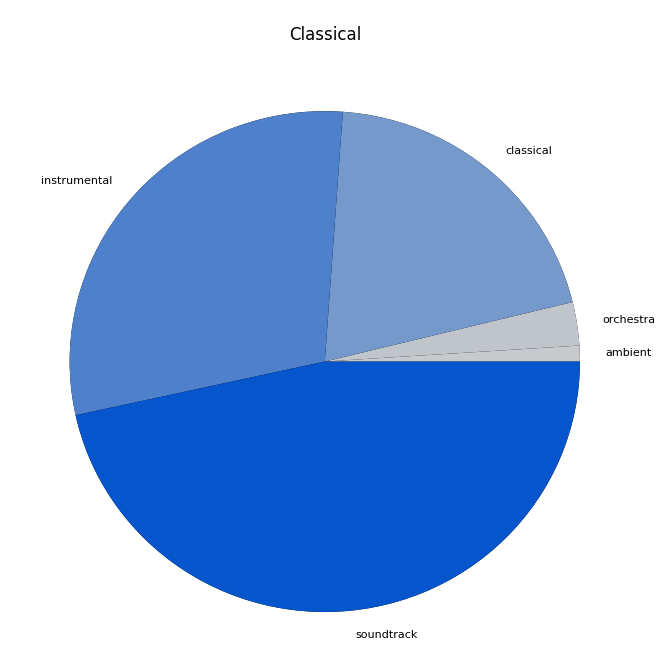
\includegraphics[height=0.45\paperheight]{src/images/classical_dist.png}
    \caption{A klasszikus gyűjtőstílus alá tartozó alstílusok eloszlása kördiagrammon.}
\end{figure}

\begin{figure}[p]
    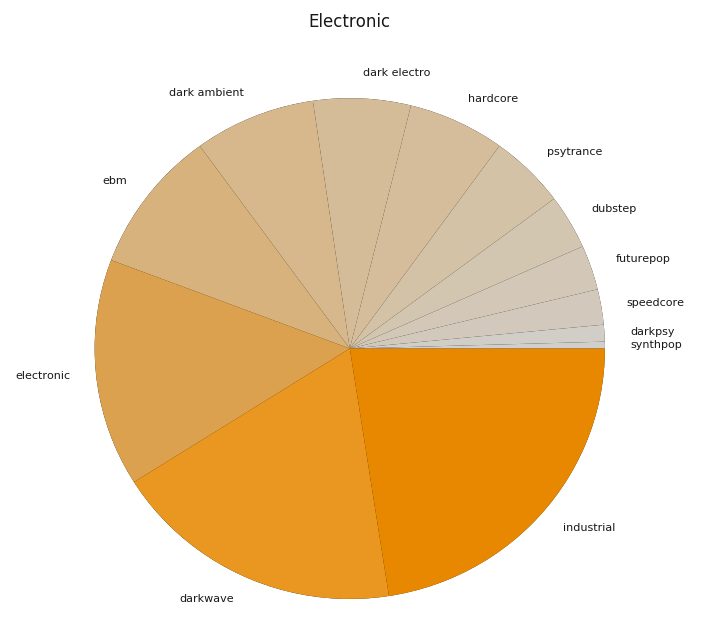
\includegraphics{src/images/electronic_dist.png}
    \caption{Az elektronikus gyűjtőstílus alá tartozó alstílusok eloszlása kördiagrammon.}
\end{figure}

\begin{figure}[p]
    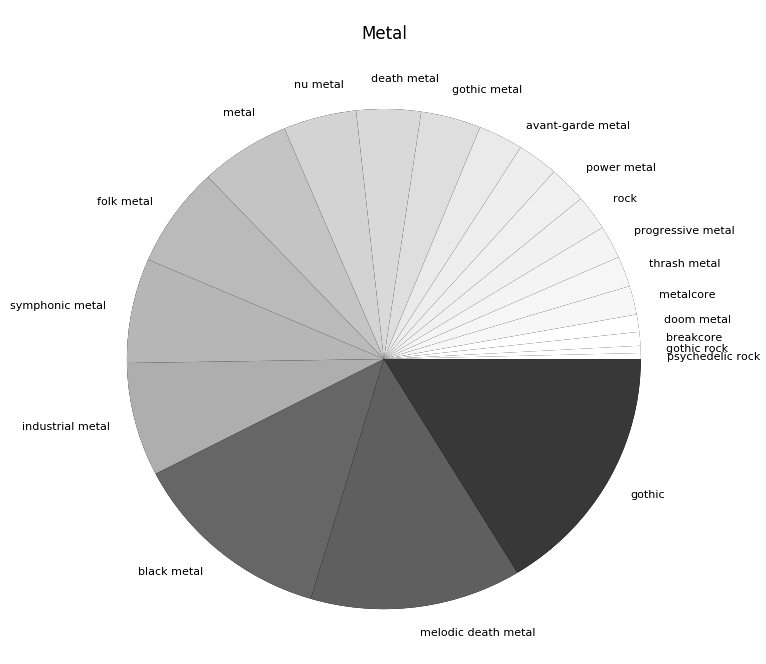
\includegraphics{src/images/metal_dist.png}
    \caption{A metál gyűjtőstílus alá tartozó alstílusok eloszlása kördiagrammon.}
\end{figure}

\begin{figure}[p]
    \centering
    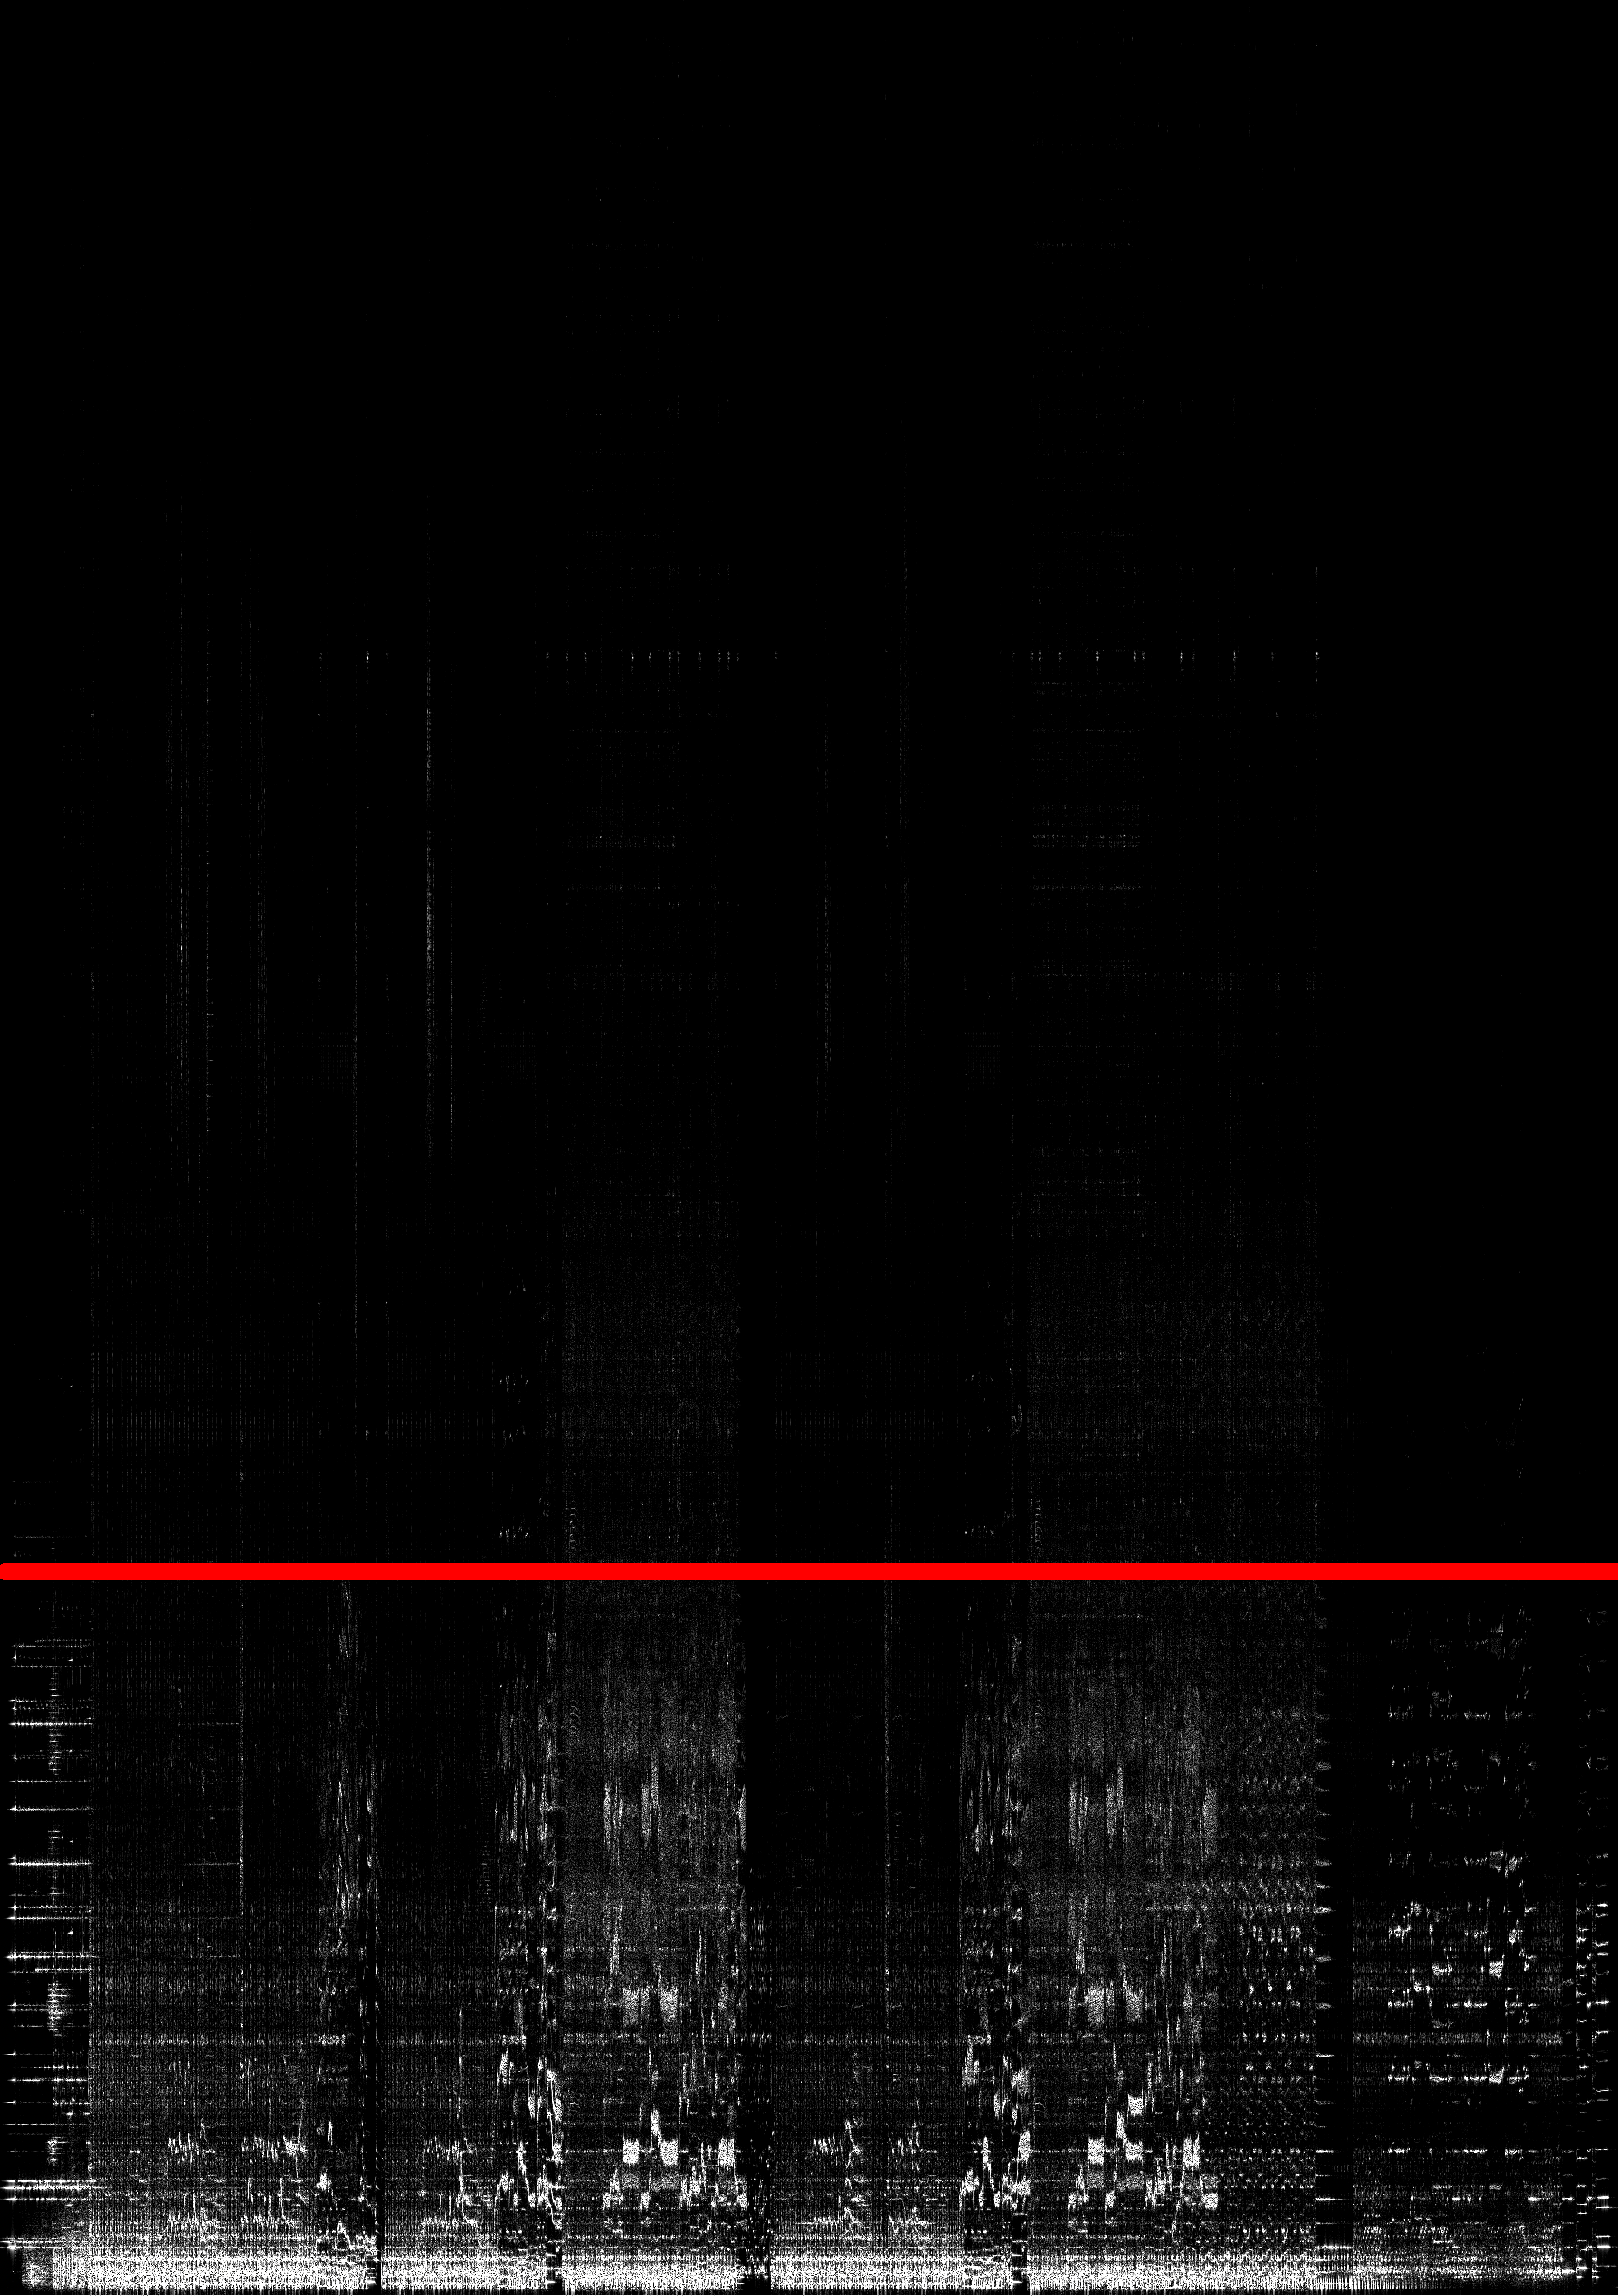
\includegraphics[height=0.75\paperheight]{src/images/DSO_Heroines.png}
    \caption{Példa egy dal spektrogramjára, melyből a megfelelő percentilisekhez tartozó szeleteket exportáltam. A piros
    vonal alatti terület jelöli a spektrogram azon részét, amit felhasználtam a spektrogramszeletek exportálásához. A spektrogram
    a Diablo Swing Orchestra előadó Heroines című dalából készült.}
\end{figure}

\begin{figure}[p]
    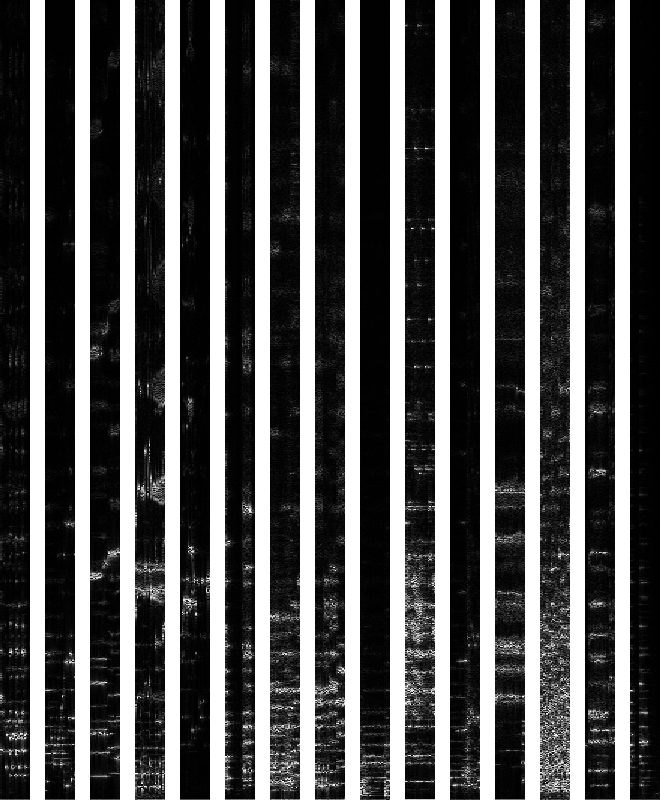
\includegraphics[height=0.80\paperheight]{src/images/example_slices_classical.png}
    \caption{Példa az adathalmaz klasszikus stílusához tartozó spektrogram szeleteiből.}
\end{figure}

\begin{figure}[p]
    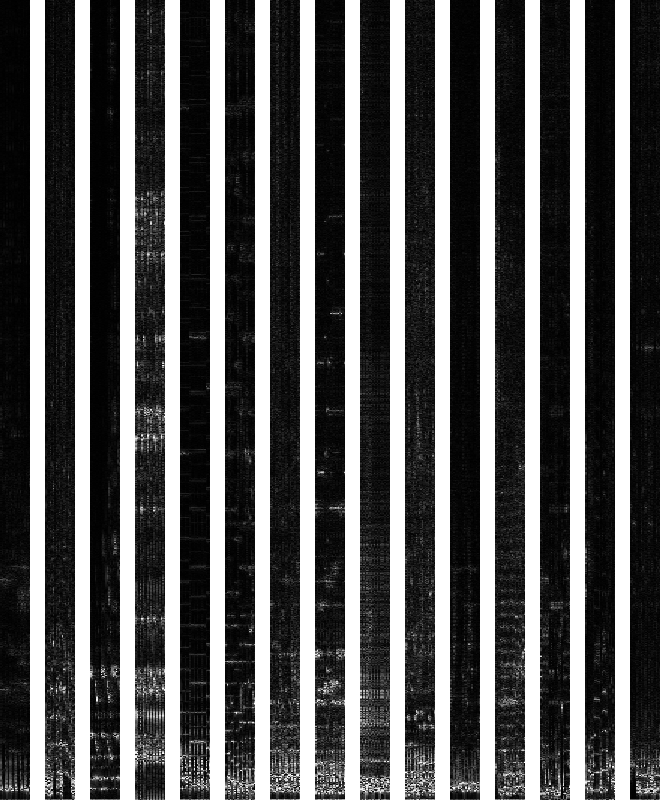
\includegraphics[height=0.80\paperheight]{src/images/example_slices_electronic.png}
    \caption{Példa az adathalmaz elektronikus stílusához tartozó spektrogram szeleteiből.}
\end{figure}

\begin{figure}[p]
    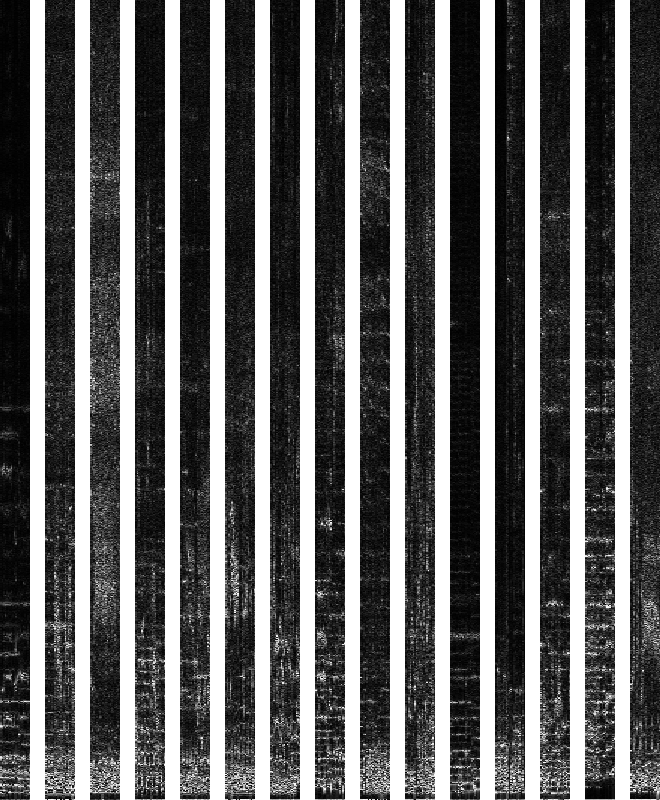
\includegraphics[height=0.80\paperheight]{src/images/example_slices_metal.png}
    \caption{Példa az adathalmaz metál stílusához tartozó spektrogram szeleteiből.}
\end{figure}

\begin{figure}[p]
    \centering
    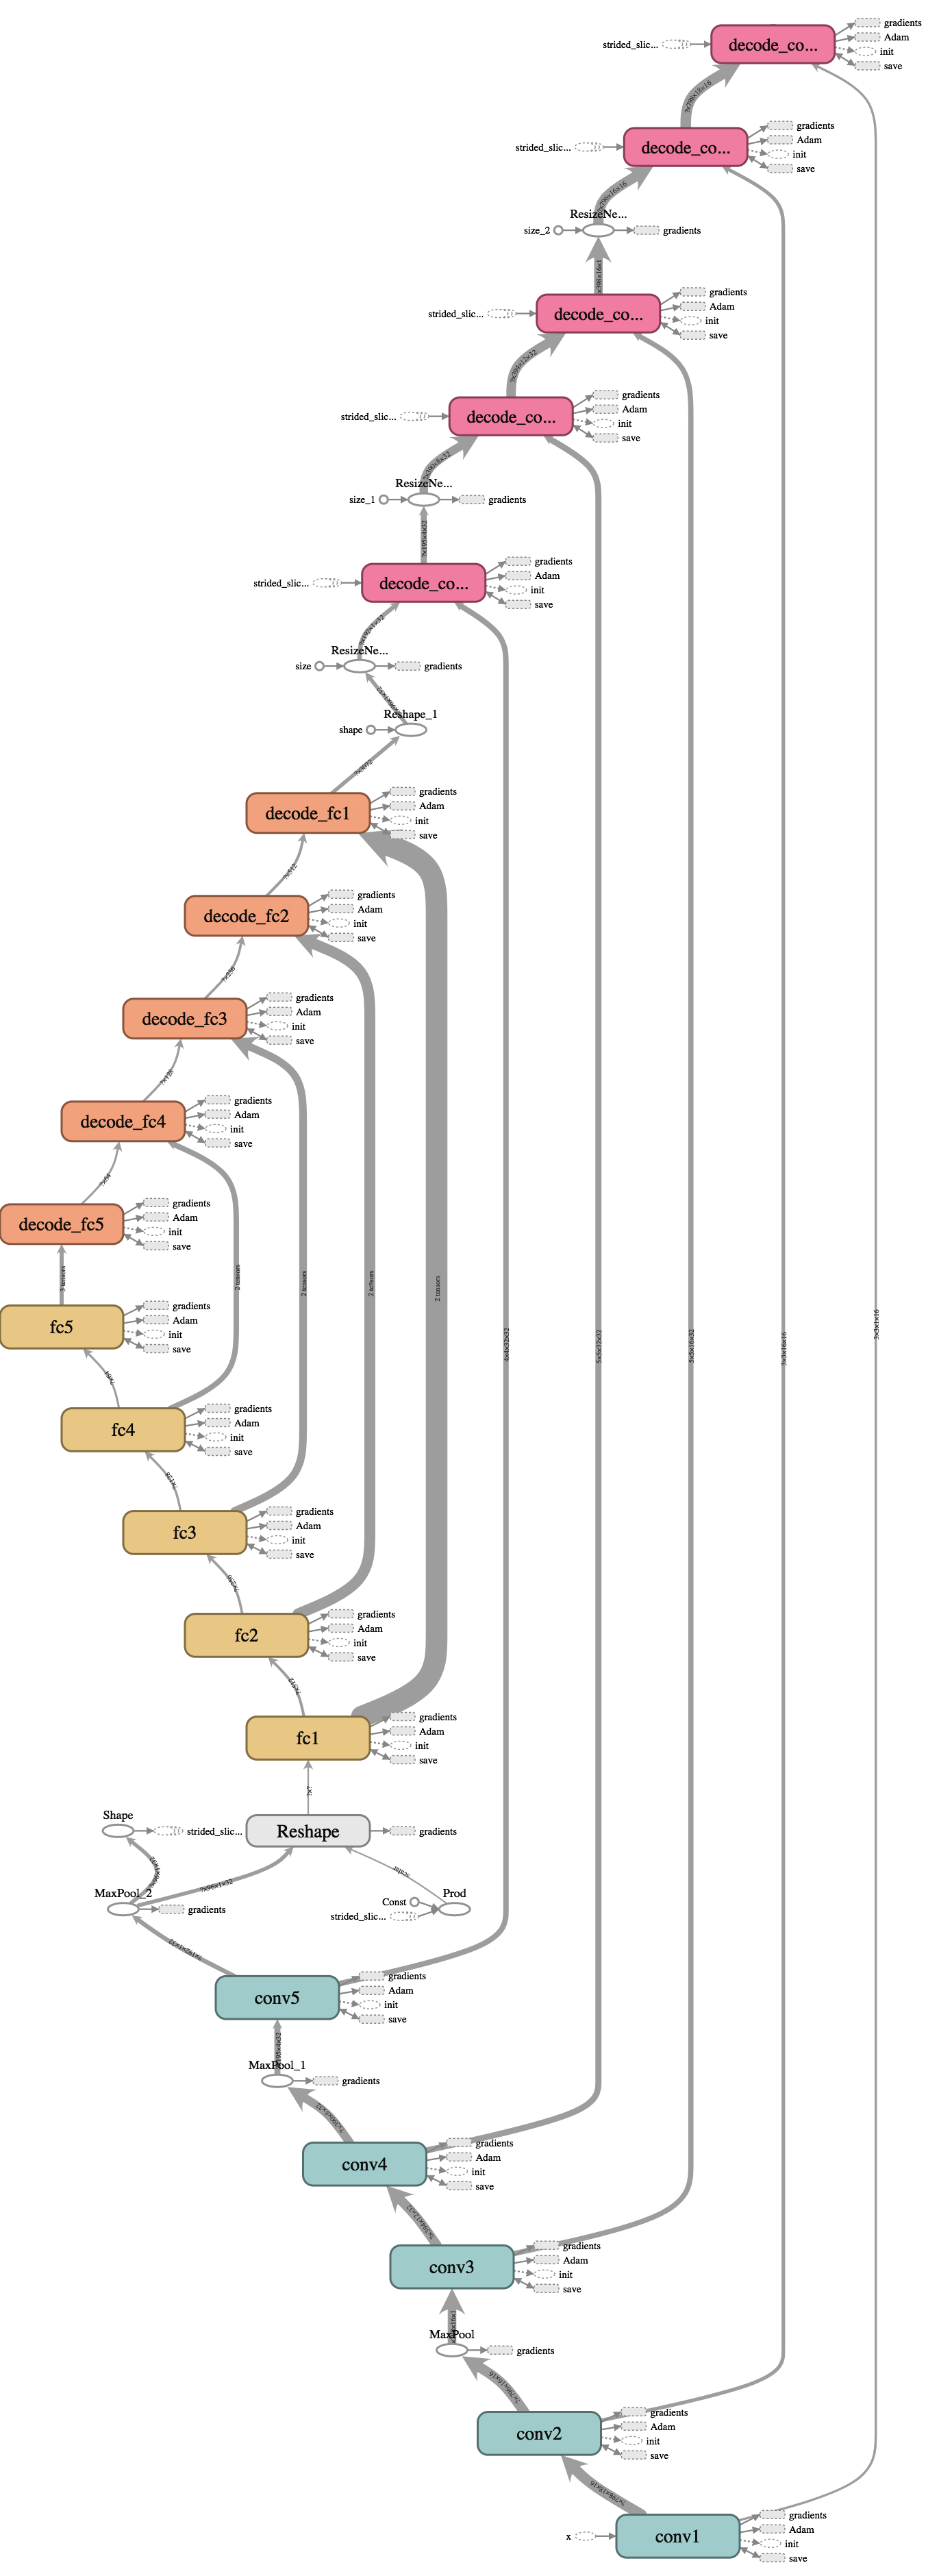
\includegraphics[height=0.70\paperheight]{src/images/tensorflow_graph_big.png}
    \caption{Az autoencoder számítási gráfja. Az encoder és decoder részek egymás tükörképei, ezt a diagram szimmetriája
    is mutatja. Alulról felfelé haladva a kék node-ok az encoder konvolúciós rétegeit, a sárgák az encoder fully connected rétegeit,
    a narancssárgák a decoder fully connected rétegeit, a rózsaszín node-ok pedig a decoder dekonvolúciós rétegeit jelölik.
    Az encoder rétegeinek megfelelő decoder rétegek az encoder rétegek súlyainak transzponáltját használják, ez a diagramon is látszik,
    hiszen a decoder rétegek közvetlenül össze vannak a nekik megfelelő encoder réteggel is.}
\end{figure}

\begin{figure}[p]
    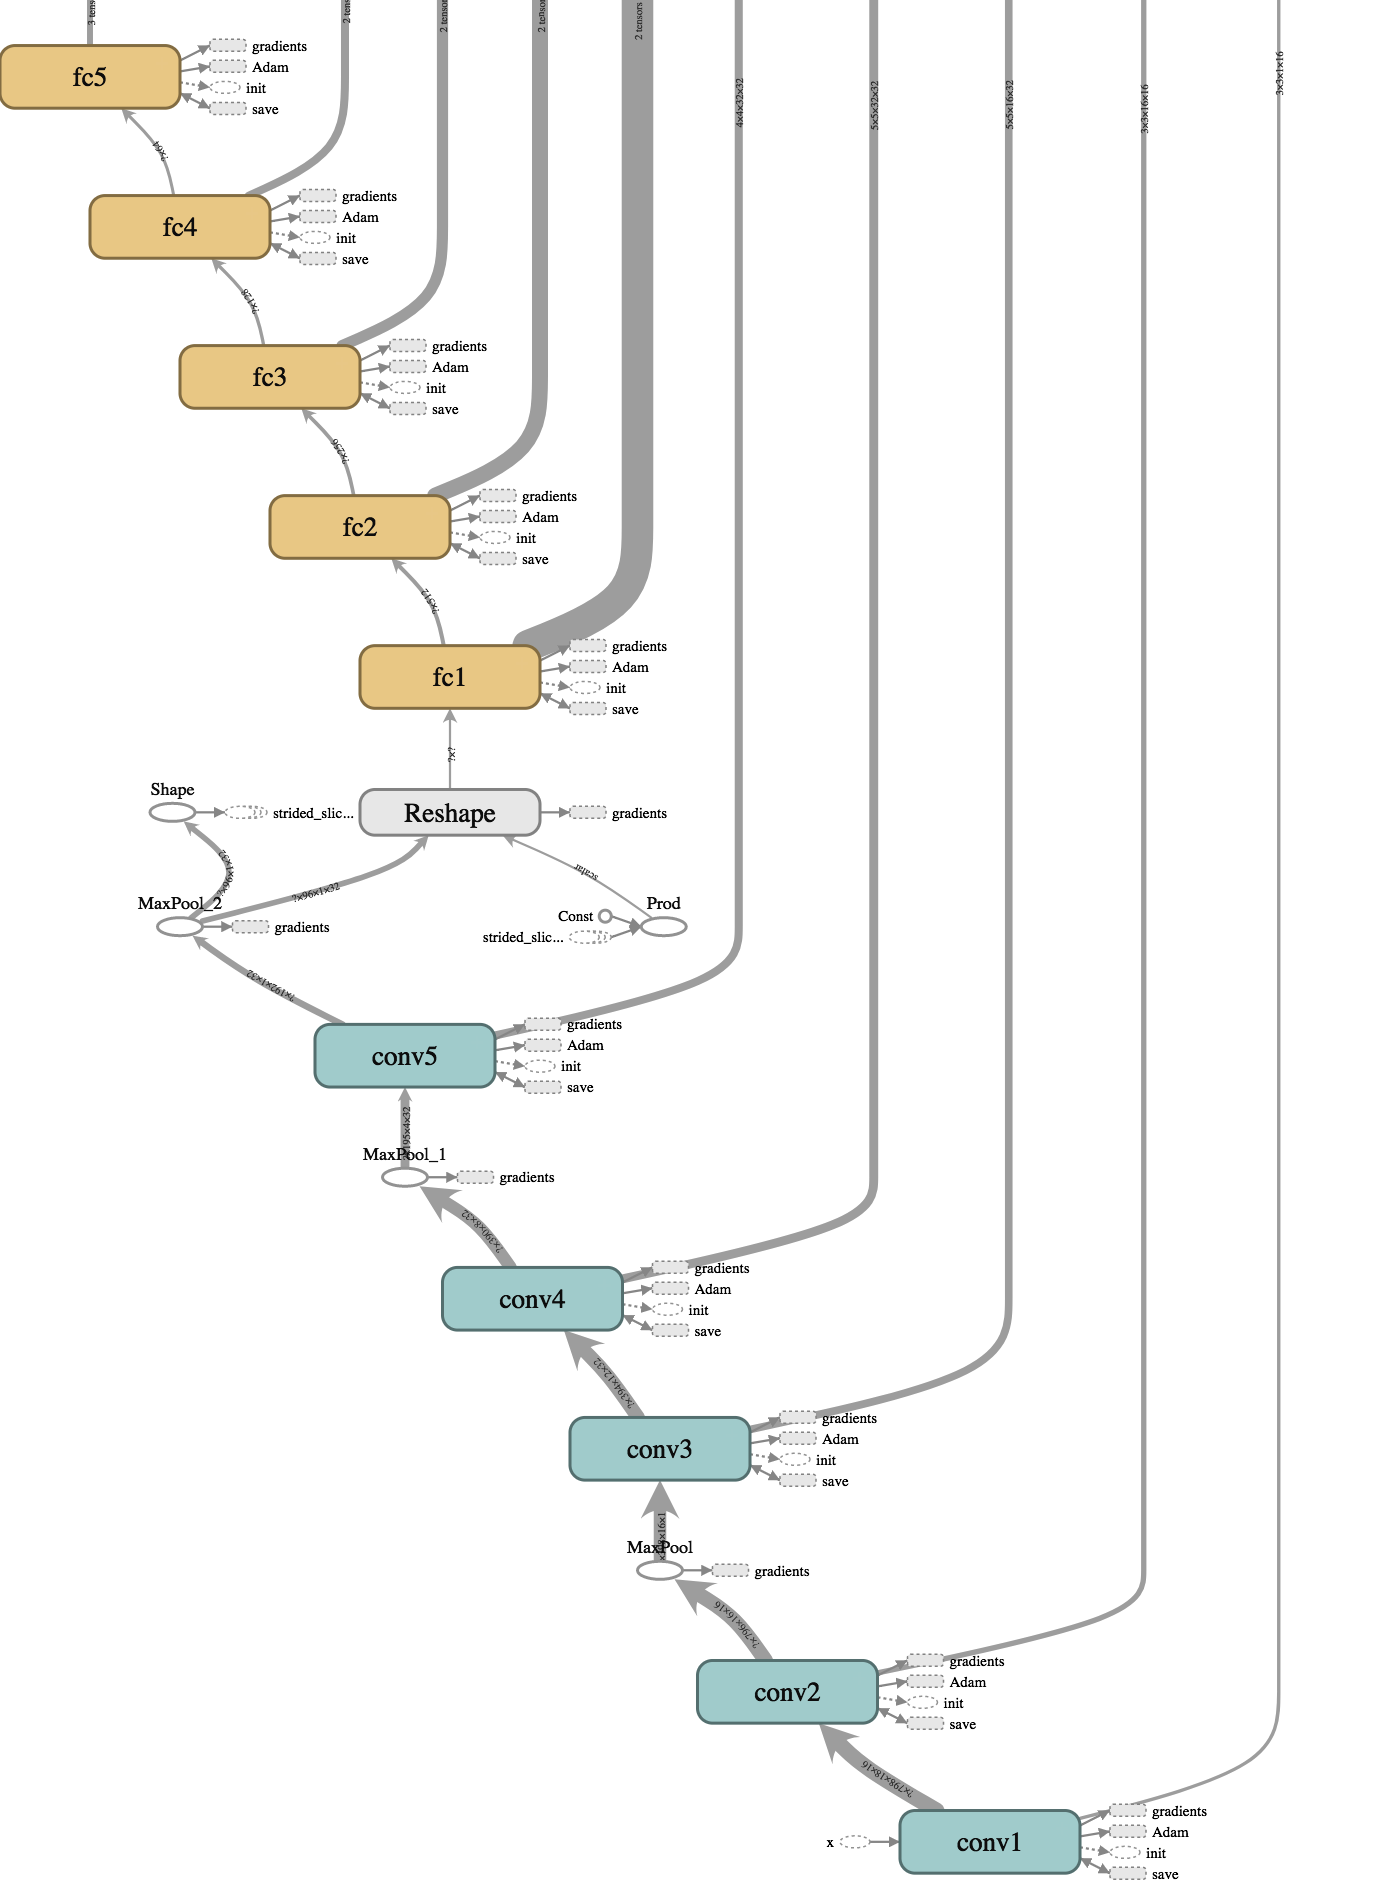
\includegraphics{src/images/tensorflow_graph_encode.png}
    \caption{A neuronháló encoder része. Az 'fc5' nevű réteg kimenete a 32-dimenziós encoding.}
\end{figure}

\begin{figure}[p]
    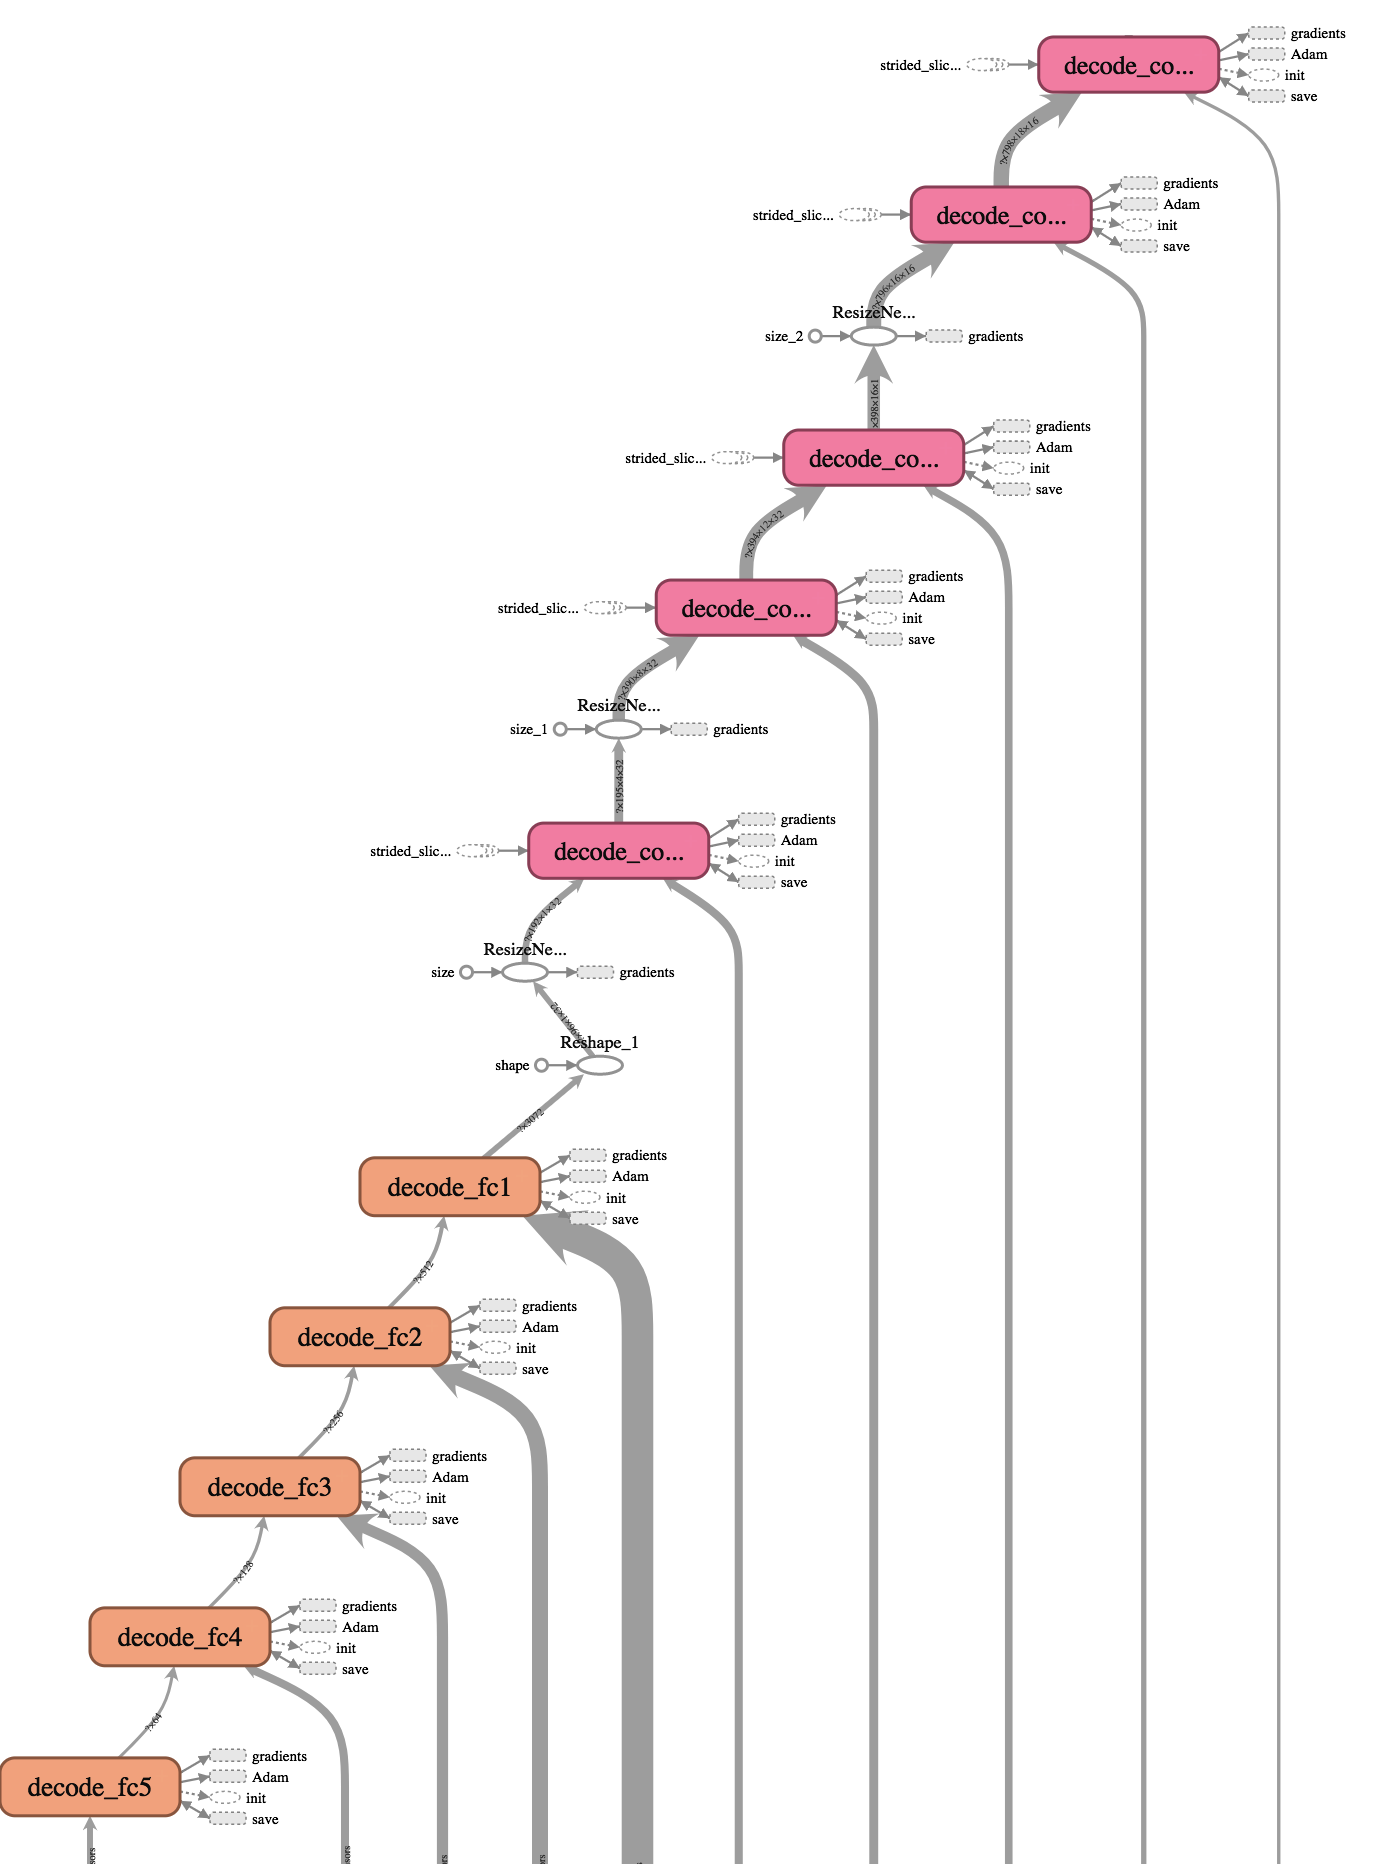
\includegraphics{src/images/tensorflow_graph_decode.png}
    \caption{A neuronháló decoder része.}
\end{figure}

\begin{figure}[p]
    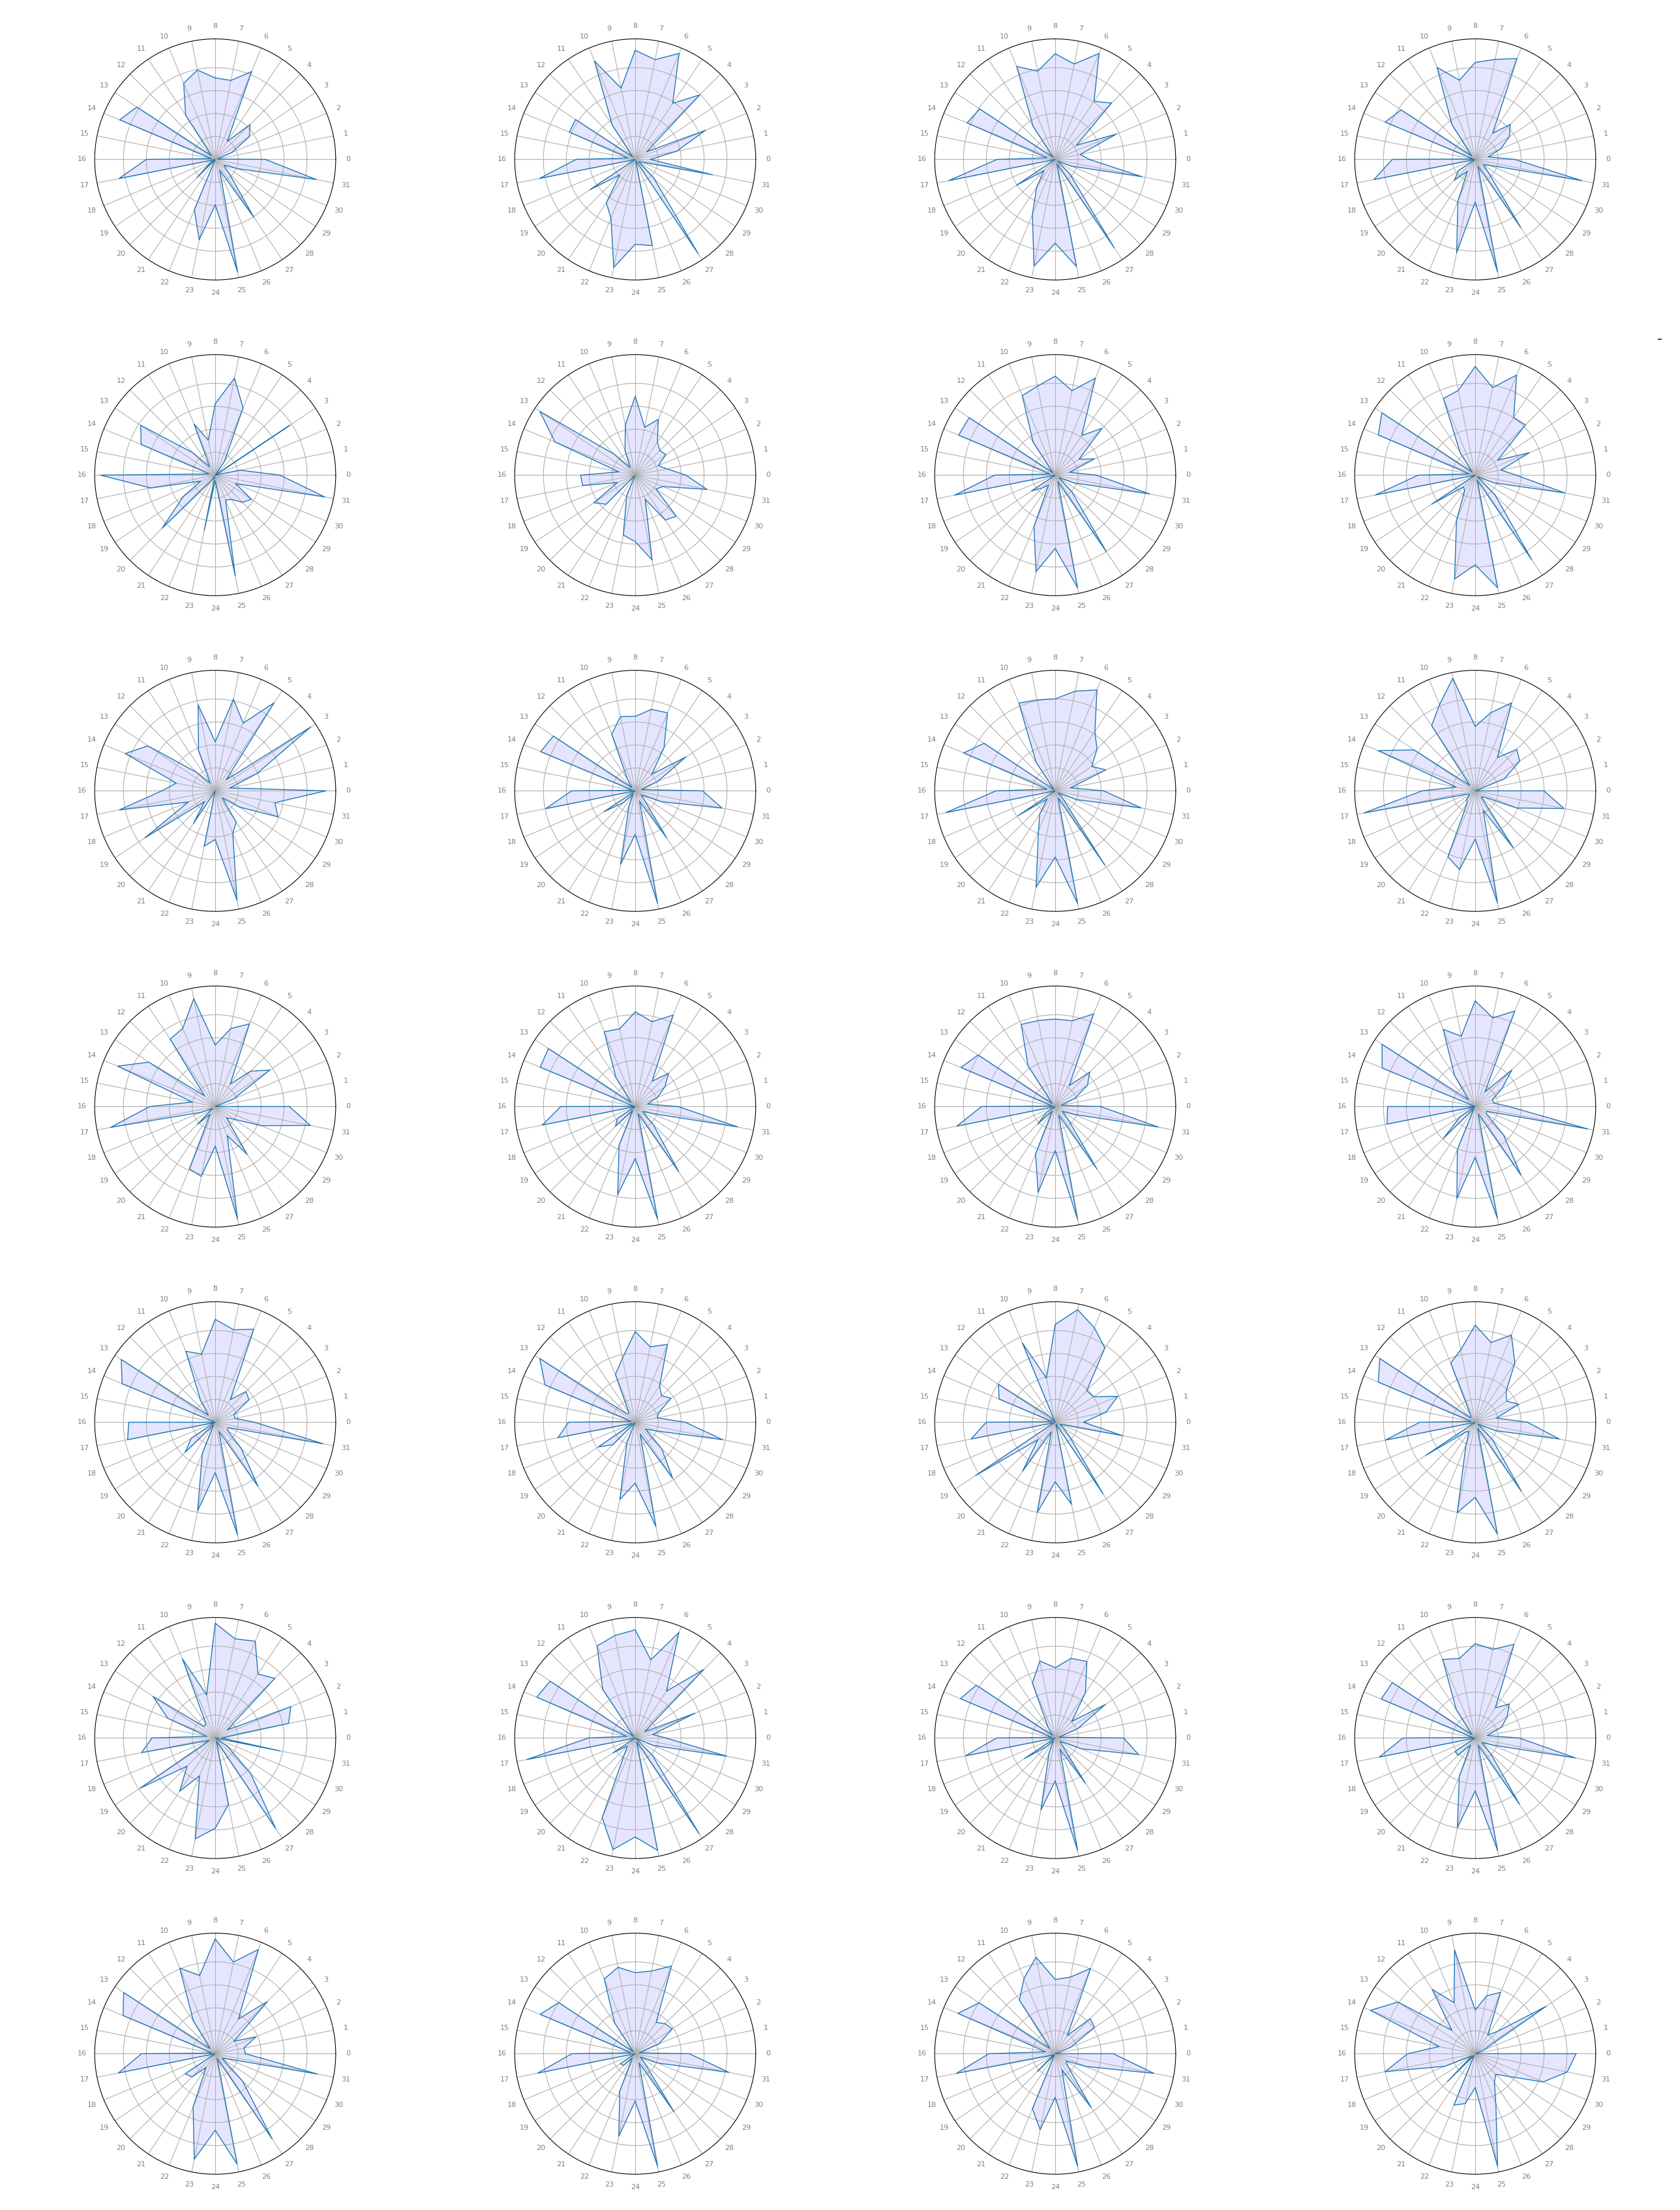
\includegraphics{src/images/radar_classical.png}
    \caption{Radar chart-ok az adathalmaz klasszikus stílusához tartozó dalokból.}
\end{figure}

\begin{figure}[p]
    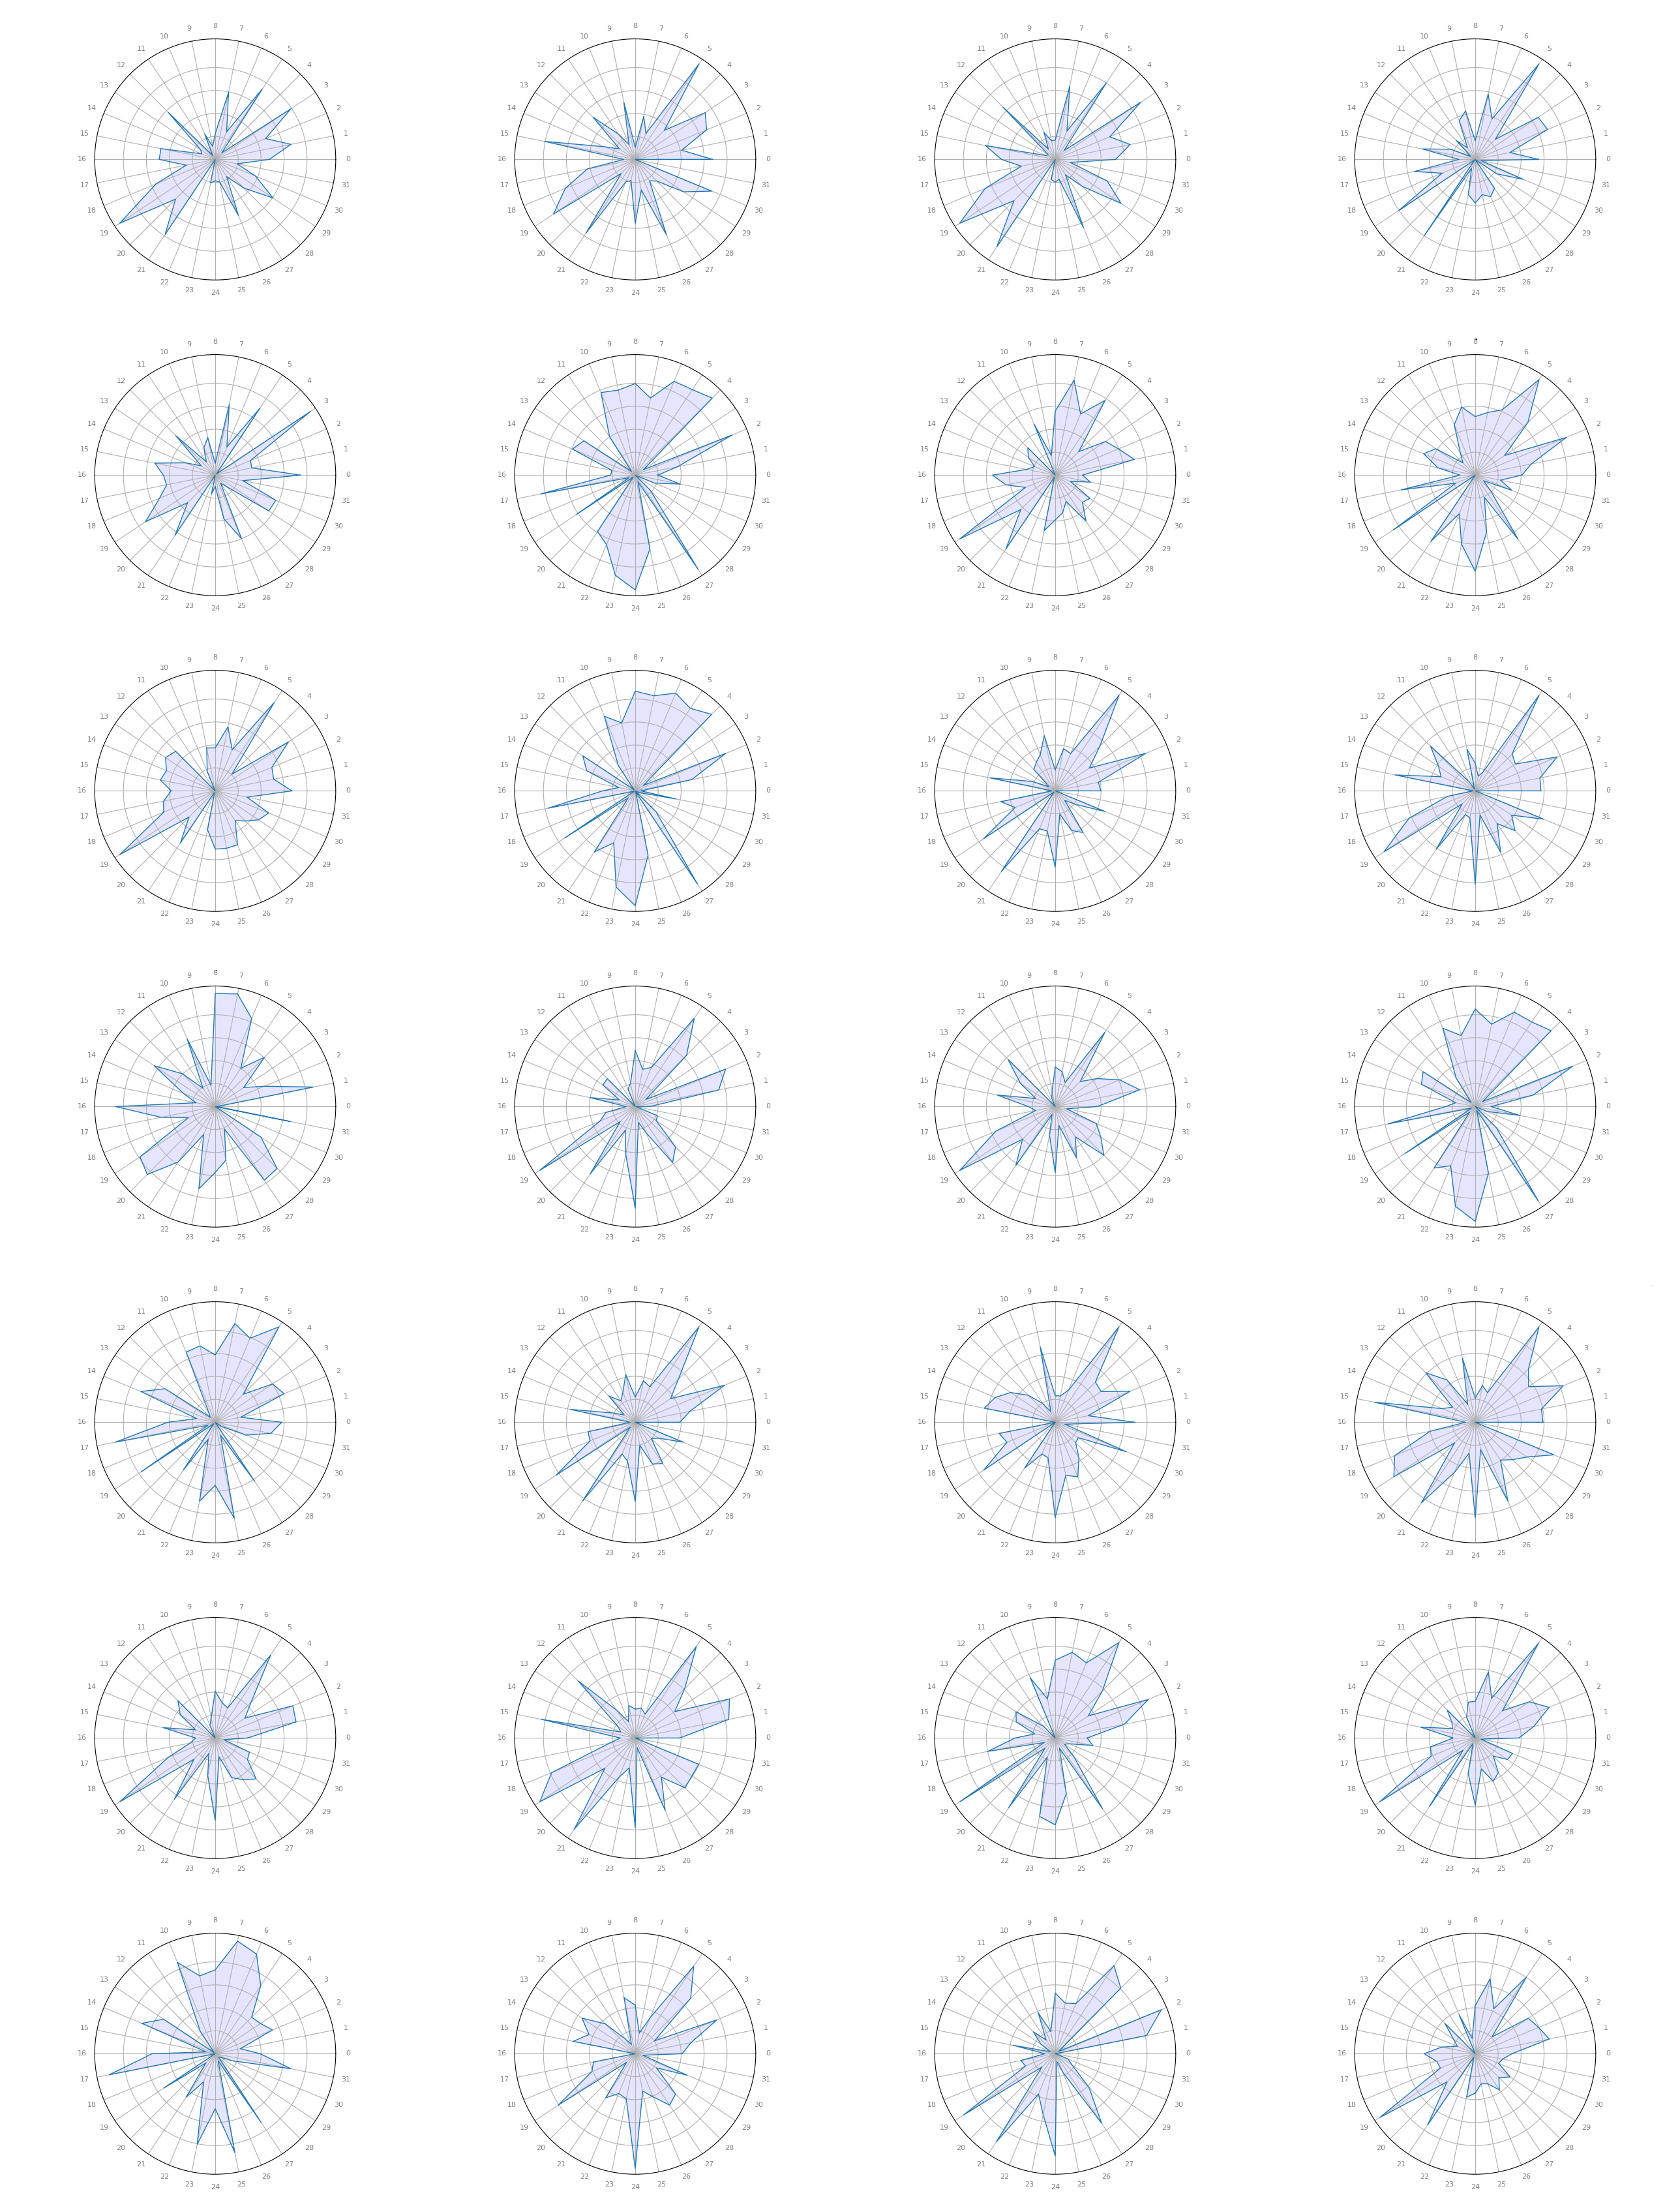
\includegraphics{src/images/radar_electronic.png}
    \caption{Radar chart-ok az adathalmaz elektronikus stílusához tartozó dalokból.}
\end{figure}

\begin{figure}[p]
    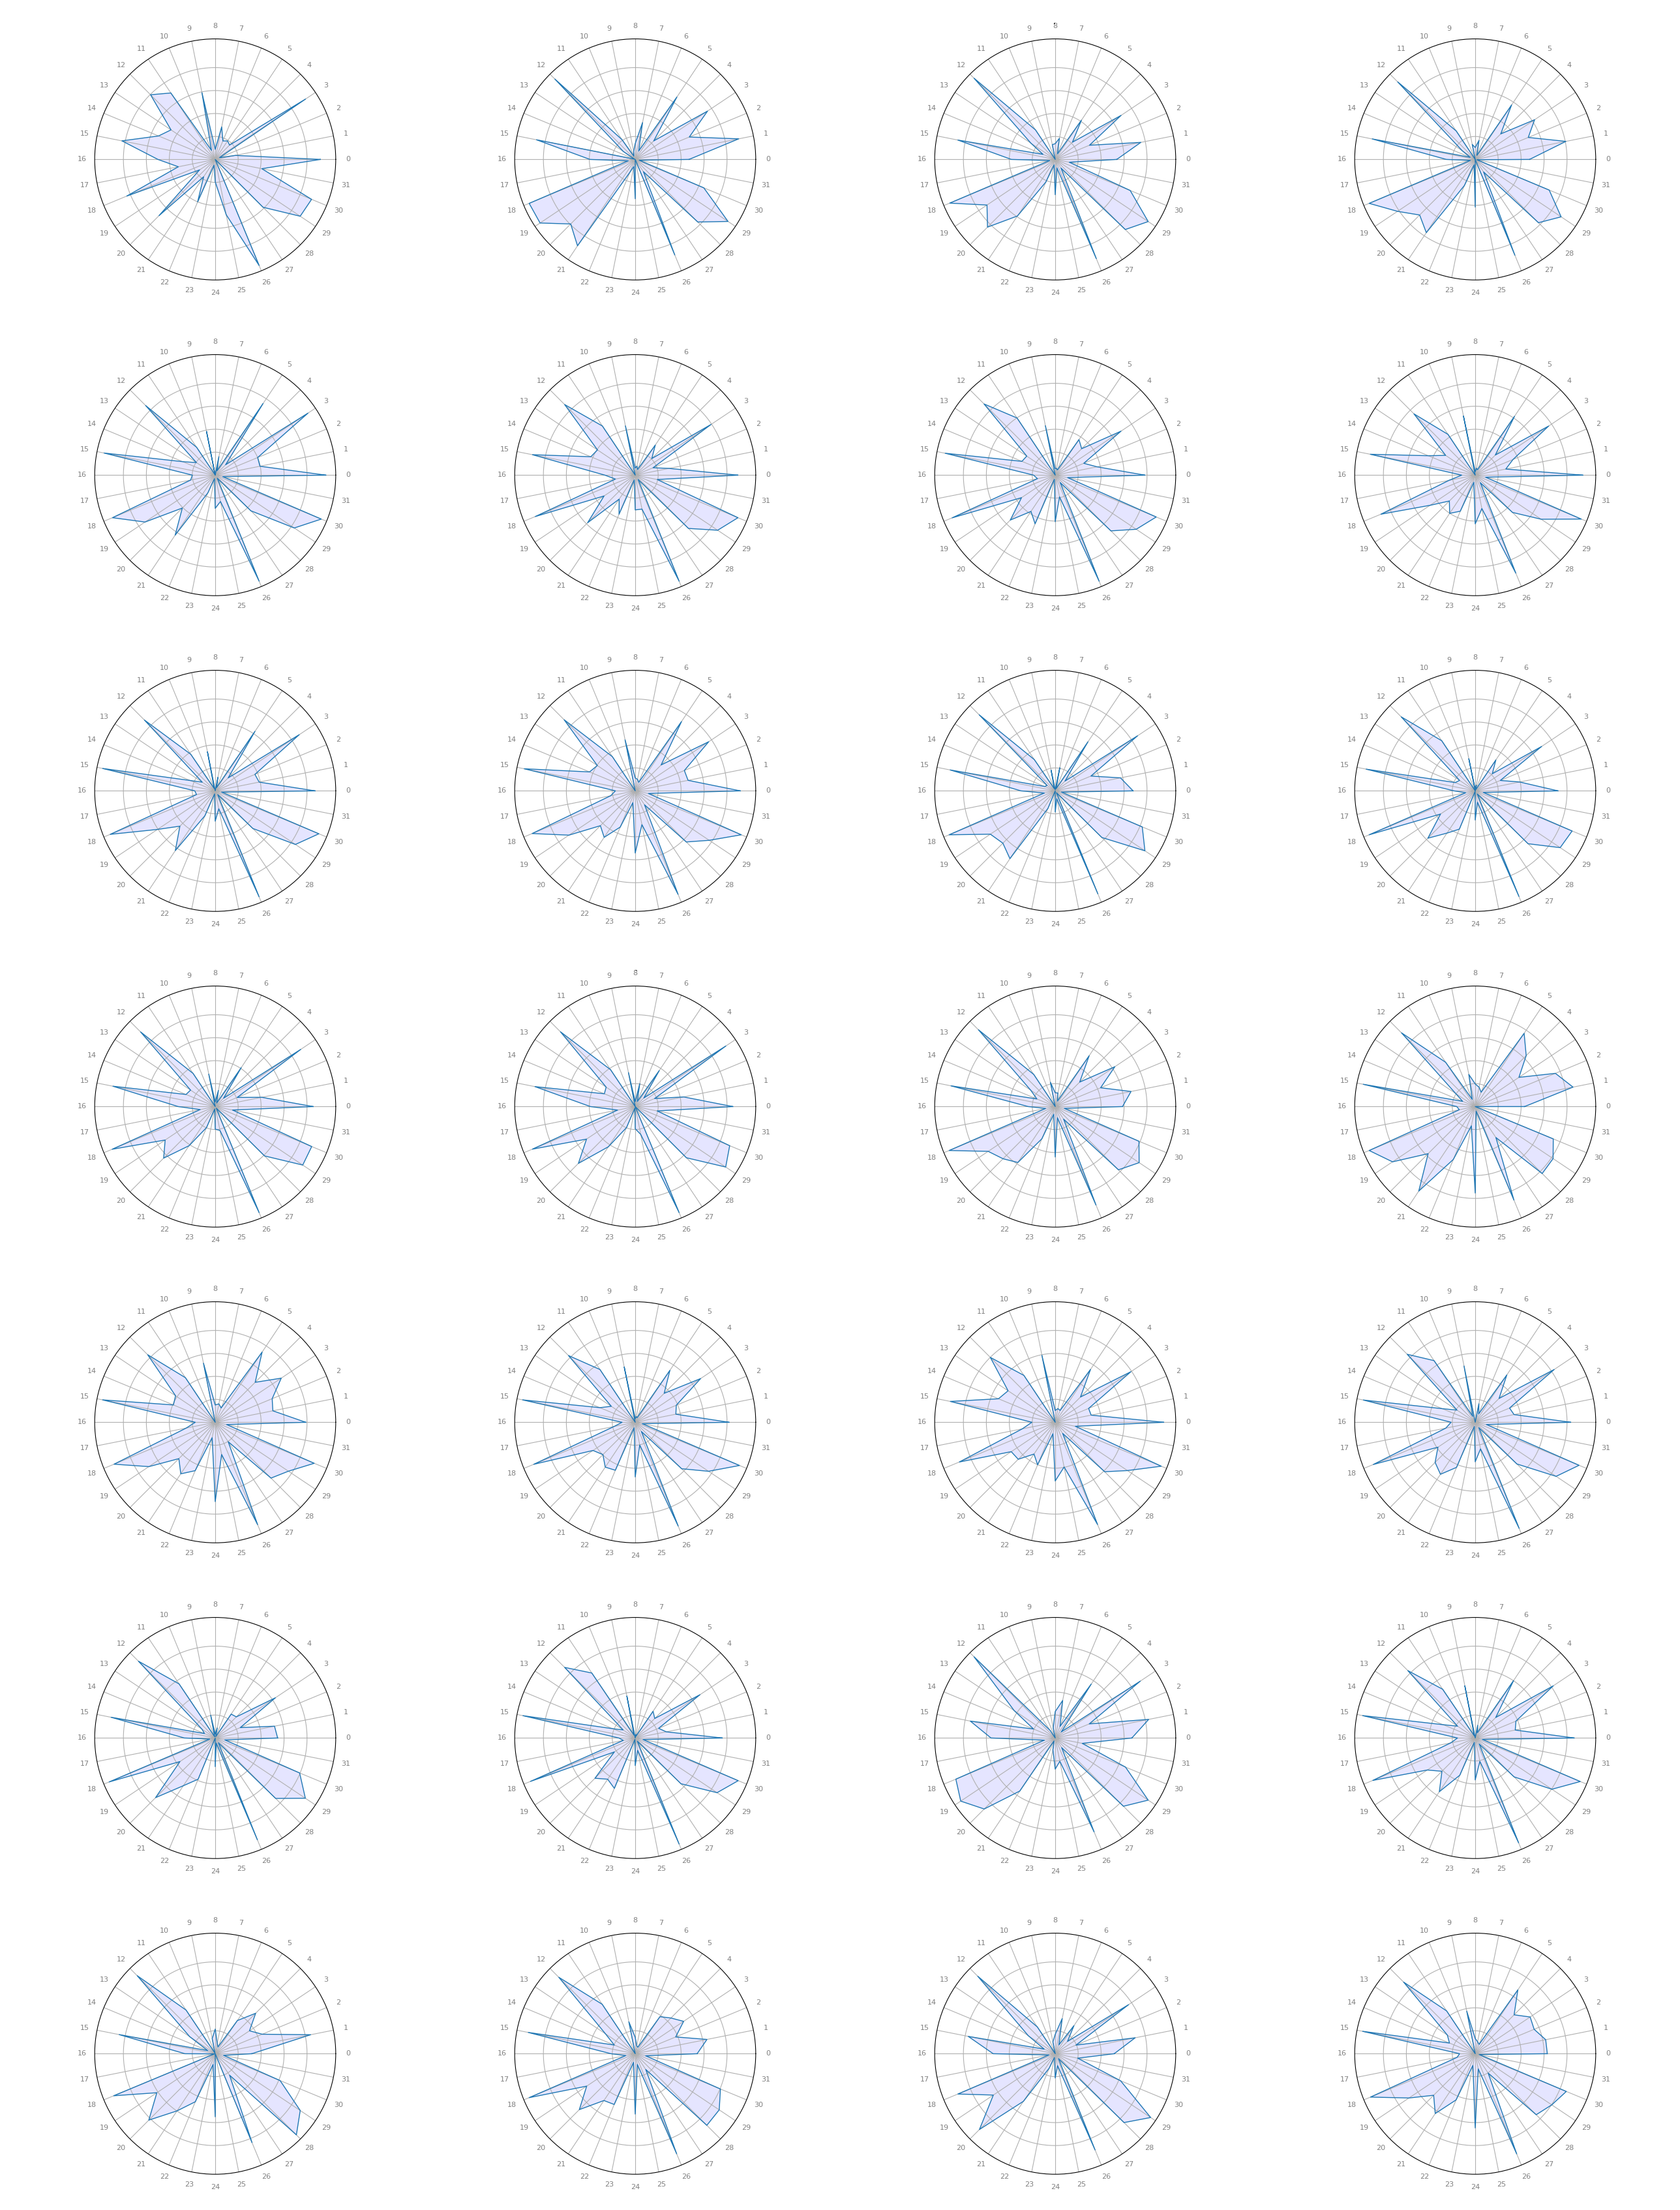
\includegraphics{src/images/radar_metal.png}
    \caption{Radar chart-ok az adathalmaz metál stílusához tartozó dalokból.}
\end{figure}

\begin{figure}[p]
    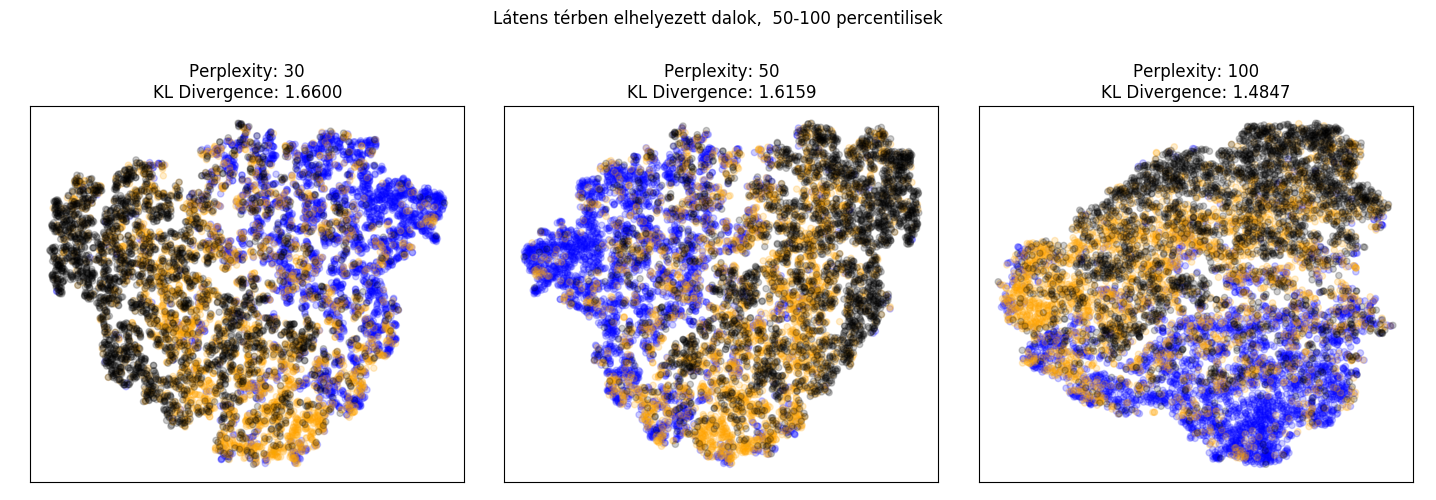
\includegraphics{src/images/tsne_extra_1.png}
    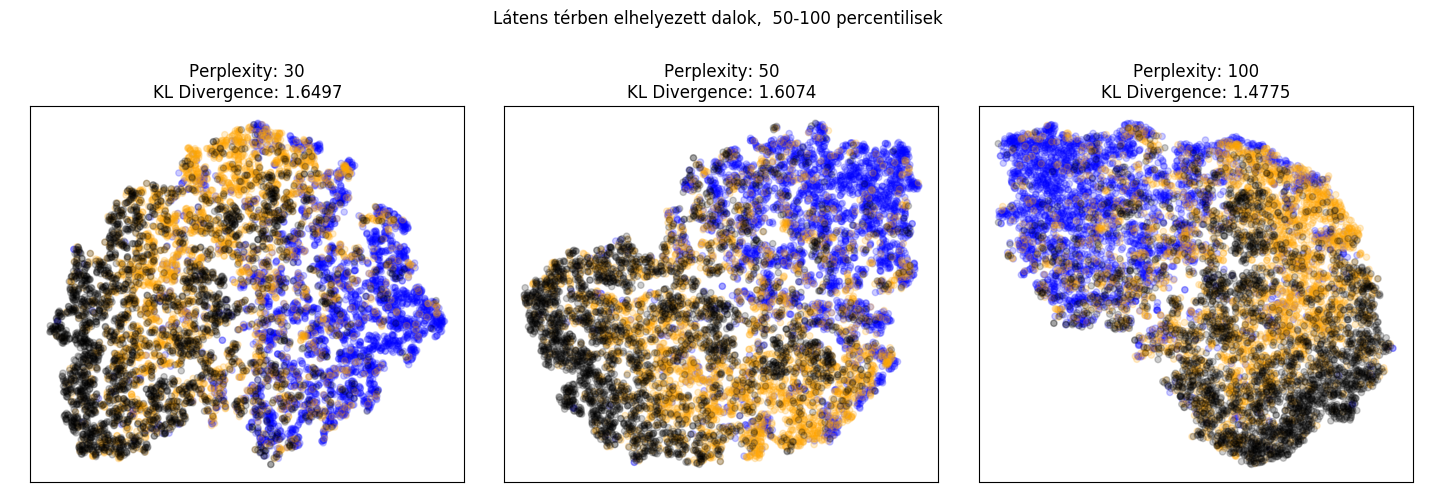
\includegraphics{src/images/tsne_extra_2.png}
    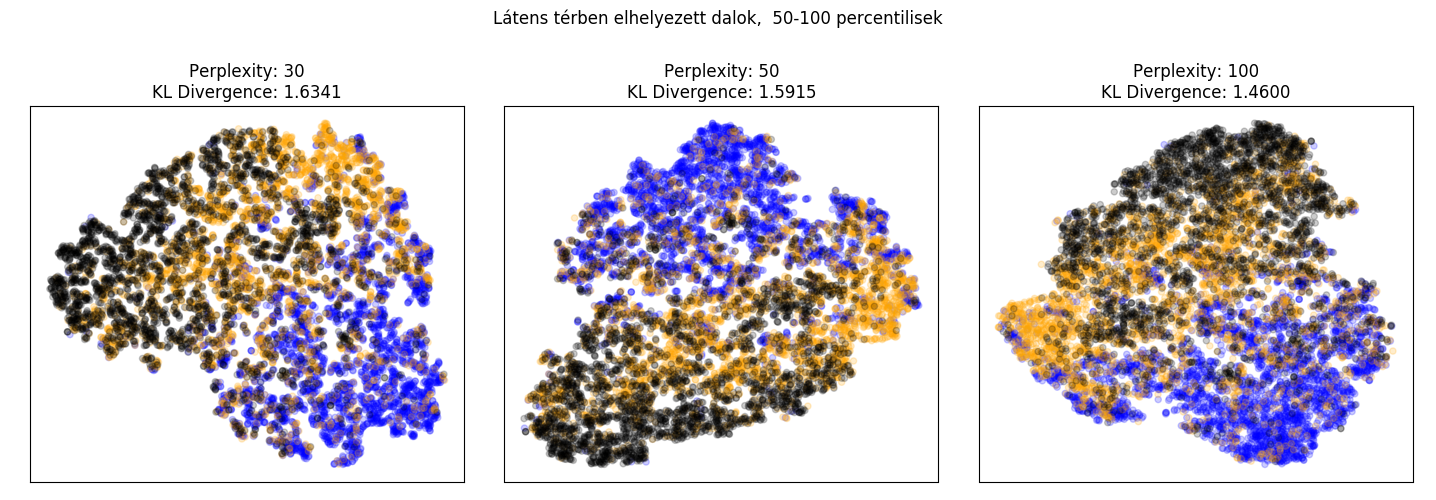
\includegraphics{src/images/tsne_extra_3.png}
    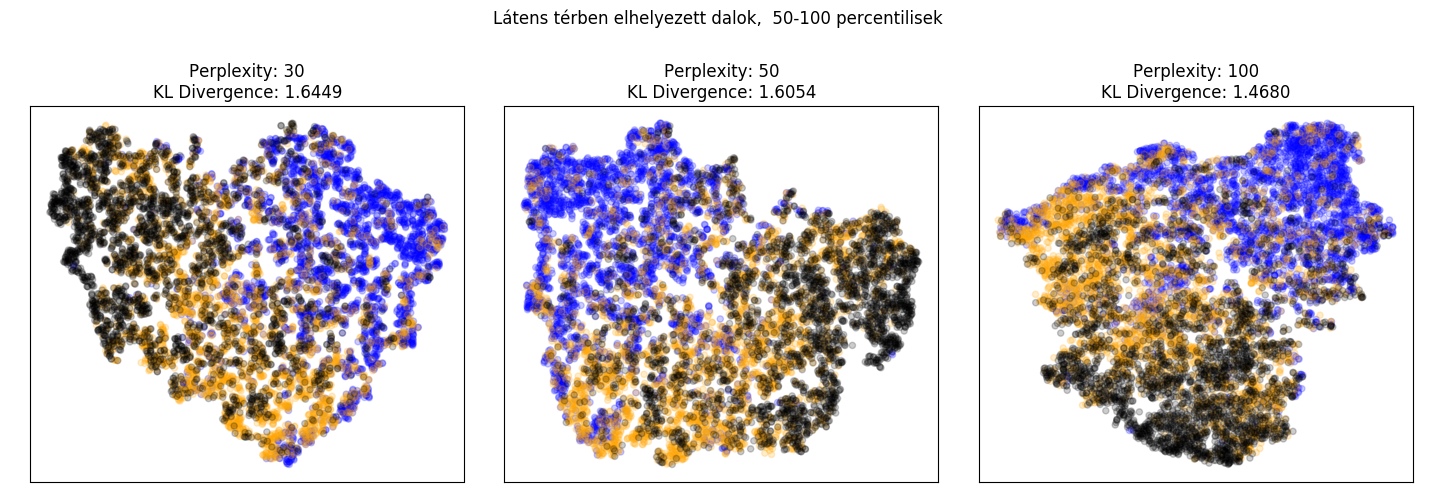
\includegraphics{src/images/tsne_extra_4.png}
    \caption{További t-SNE vizualizációk eredményei, stílusonként 3000 pontra nézve, különböző perplexity értékekkel (30, 50, 100).}
\end{figure}

\pagebreak
\footnotesize\csvautolongtable[
table head={
\hline \rowcolor{black!15} \# & Stílus & Előadó & Dal & Percentilis \\\hline
\endfirsthead
\hline
\caption{Egy főképp klasszikus címkéjű dalokat tartalmaző lejátszási lista. A lista végén megfigyelhető, ahogy a lejátszási
lista generáló algoritmus
átnavigált a látens tér elektronikus területére.}
\endfoot
},
respect all
]{src/tables/appendix_playlist_classical.csv}\normalsize

\pagebreak
\footnotesize\csvautolongtable[
table head={
\hline \rowcolor{black!15} \# & Stílus & Előadó & Dal & Percentilis \\\hline
\endfirsthead
\hline
\caption{Javarészt elektronikus dalokból álló lejátszási lista egy rövidebb klasszikus intermezzo-val a 22. daltól.}
\endfoot
},
respect all
]{src/tables/appendix_playlist_electronic.csv}\normalsize

\pagebreak
\footnotesize\csvautolongtable[
table head={
\hline \rowcolor{black!15} \# & Stílus & Előadó & Dal & Percentilis \\\hline
\endfirsthead
\hline
\caption{Többnyire metál dalokat tartalmazó lejátszási lista.}
\endfoot
},
respect all
]{src/tables/appendix_playlist_metal.csv}\normalsize

\pagebreak
\footnotesize\csvautolongtable[
table head={
\hline \rowcolor{black!15} \# & Stílus & Előadó & Dal & Percentilis \\\hline
\endfirsthead
\hline
\caption{Elektronikus és metál dalokat vegyesen tartalmazó lejátszási lista. Az algoritmus kiindulási pontja közel helyezkedhetett
el a két stílus határához, ezért tapasztalható a két stílus közötti váltakozás.}
\endfoot
},
respect all
]{src/tables/appendix_playlist_alternate.csv}\normalsize